\chapter{Evaluation}
\label{chapter:evaluation}

\section{Calibration quality}
Another tool from the same ROS Camera Calibration package is used to compute the camera calibration error.
It continuously outputs a reprojection $\mathsf{RMS}$ (Root Mean Squared) error, which is defined as
\begin{equation}
    \mathsf{RMS}(x) = \sqrt{\frac{\sum_{i=1}^{N}{(x_i - \hat{x}_i)^2}}{N}}
\end{equation}
where $x$ is one measured data sample from the experiment, $\hat{x}$ is a ground-truth data, and $N$ is a sample size.
After launching this tool, a pattern was been moved in front of each camera to collect data and analyse it.
The reprojection error varies depending on the pose of the chessboard but, in general, is quite stable, see \autoref{tab:camcalib_eval}.

\begin{table}[ht]
    \begin{center}
      \begin{tabular}{ ll l l }
      \hline
      && Left camera & Right camera \\ \hline
      Mean of RMS reprojection error & [px] & 0.06323214286 & 0.05357391304 \\
      Variance of RMS reprojection error & [px] & 0.00001159968 & 0.00002222914 \\
      \end{tabular}
    \end{center}
    \caption{RMS reprojection error of the ROS Camera Calibration results.}
    \label{tab:camcalib_eval}
\end{table}

\section{Triangulation quality}
Two experiments were conducted to measure the triangulation quality.
The same pattern with visible key points in a featureless environment was used.
Process of the experiment is shown in \autoref{fig:exp_process}.

\subsection{Experiment setup}
\label{sec:eval_setup}

\begin{figure}[ht]
    \centering
    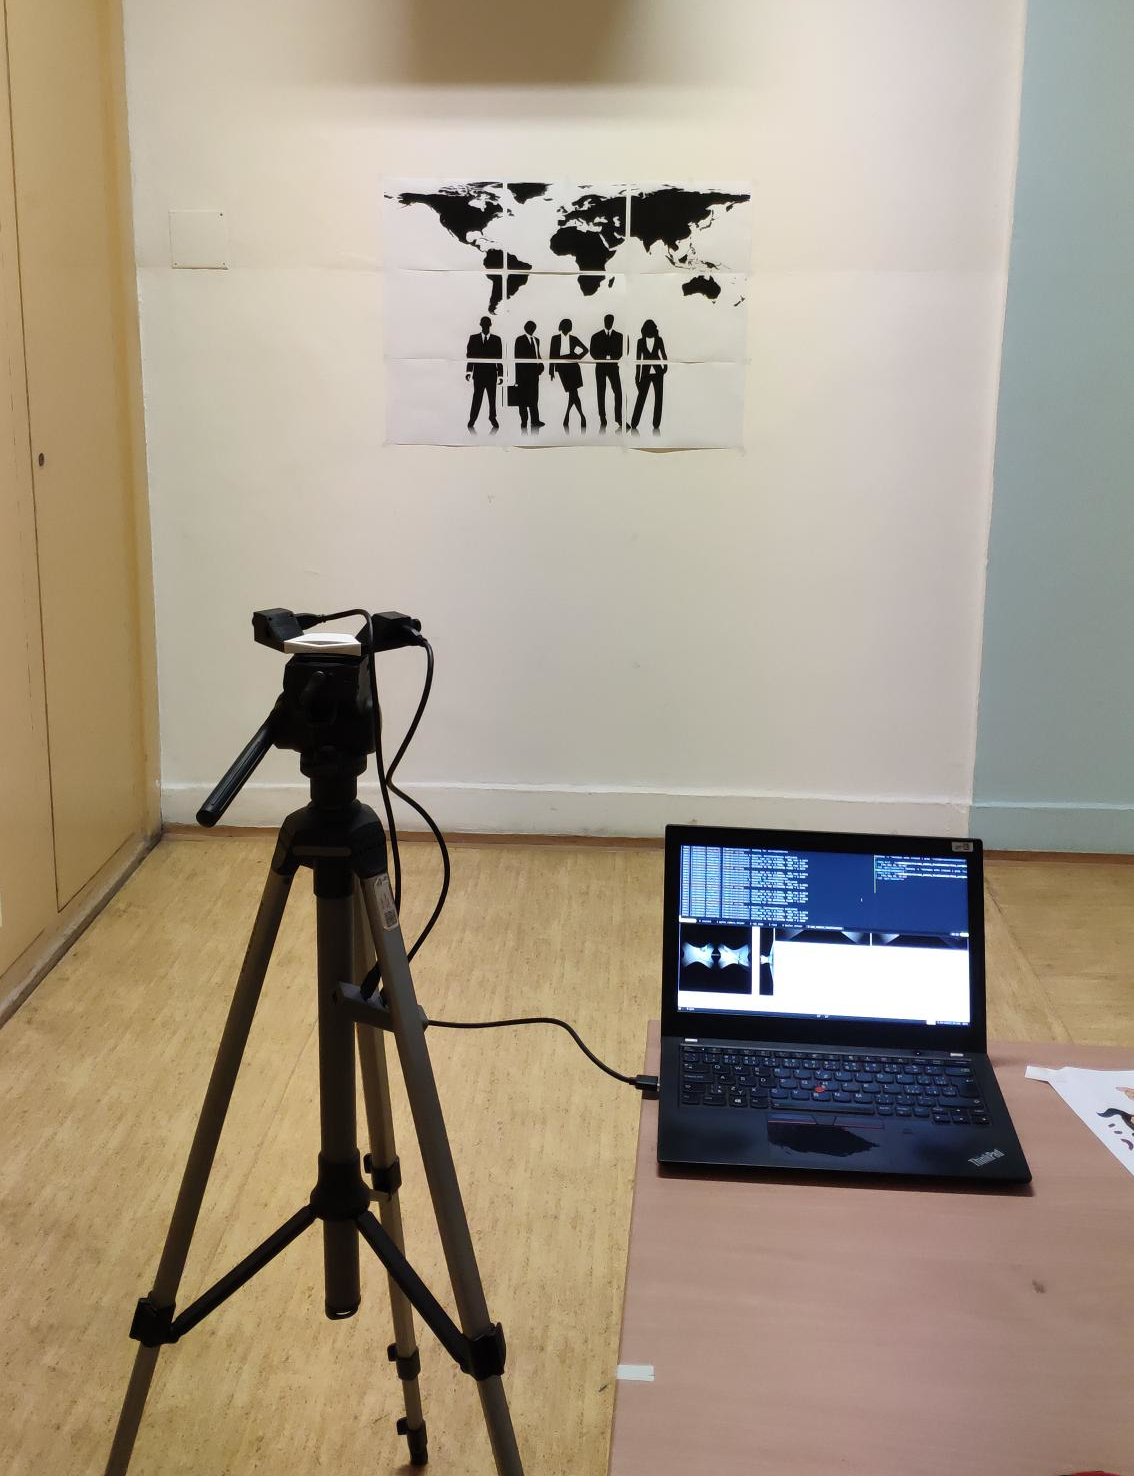
\includegraphics[width=0.6\textwidth]{graphics/experiment_setup.png}
    \caption[The setup for experiments]{The setup for experiments. 
    The designed prototype is located on a tripod, at distance $d$ from the plane $\Omega$ with visual features.
    The with $Y-Z$ plane of the cameras' common coordinate frame is parallel with $\Omega$. 
    A set of 9 A4 papers with features was used to make $\Omega$ distinguishable.}
    \label{fig:exp_process}
\end{figure}

\begin{figure}[ht]
  \begin{subfigure}[t]{0.48\textwidth}
        \centering
        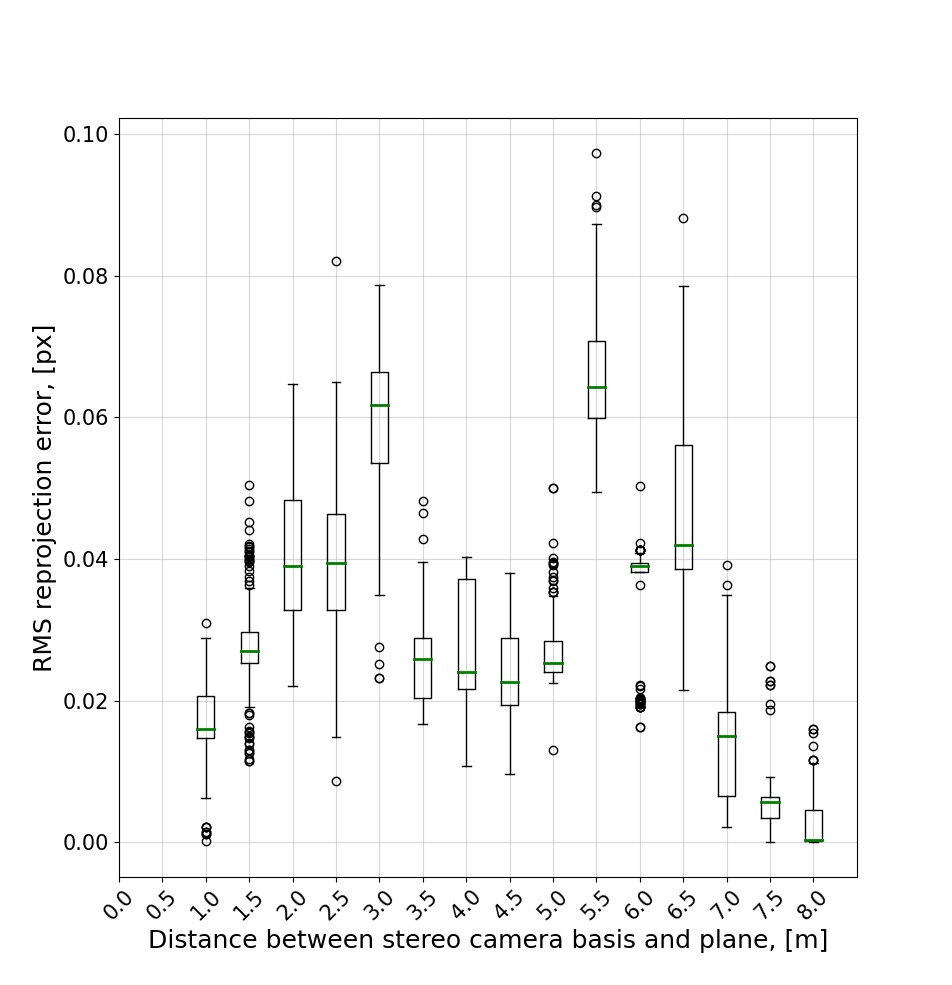
\includegraphics[width=\textwidth]{graphics/experiment_1_repro_error.png}
        \caption[Stereo pair setup RMS reprojection error.]{Stereo pair setup RMS reprojection error.}
        \label{fig:exp_1_repro}
    \end{subfigure}
    \begin{subfigure}[t]{0.48\textwidth}
        \centering
        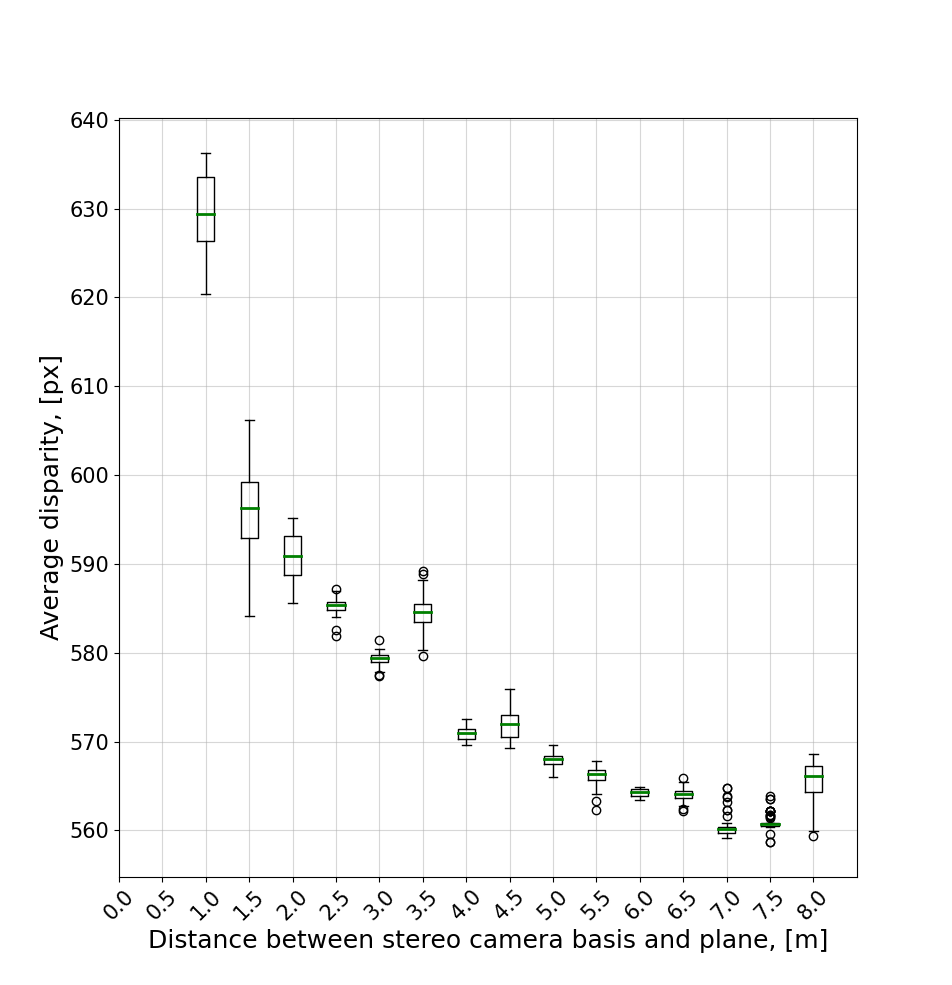
\includegraphics[width=\textwidth]{graphics/disparity_mean.png}
        \caption[Average disparity.]{Average disparity for all detected keypoints. 
        Disparity is a difference between coordinates of two matched feature points in an image pair.}
        \label{fig:exp_1_disparity}
    \end{subfigure}
  \label{fig:exp_1_res}
  \caption[The reprojection error.]{
        Green lines represents the median for each $n$ measurements at a distance $d$. 
        A box marks an interval from the first quartile to the third quartile.
        The whiskers go from each quartile of the measured values to the lower and upper fences.
        Black points represents outliers.
  }
\end{figure}

\begin{figure}[ht]
  \begin{subfigure}[ht]{0.49\textwidth}
    \centering
    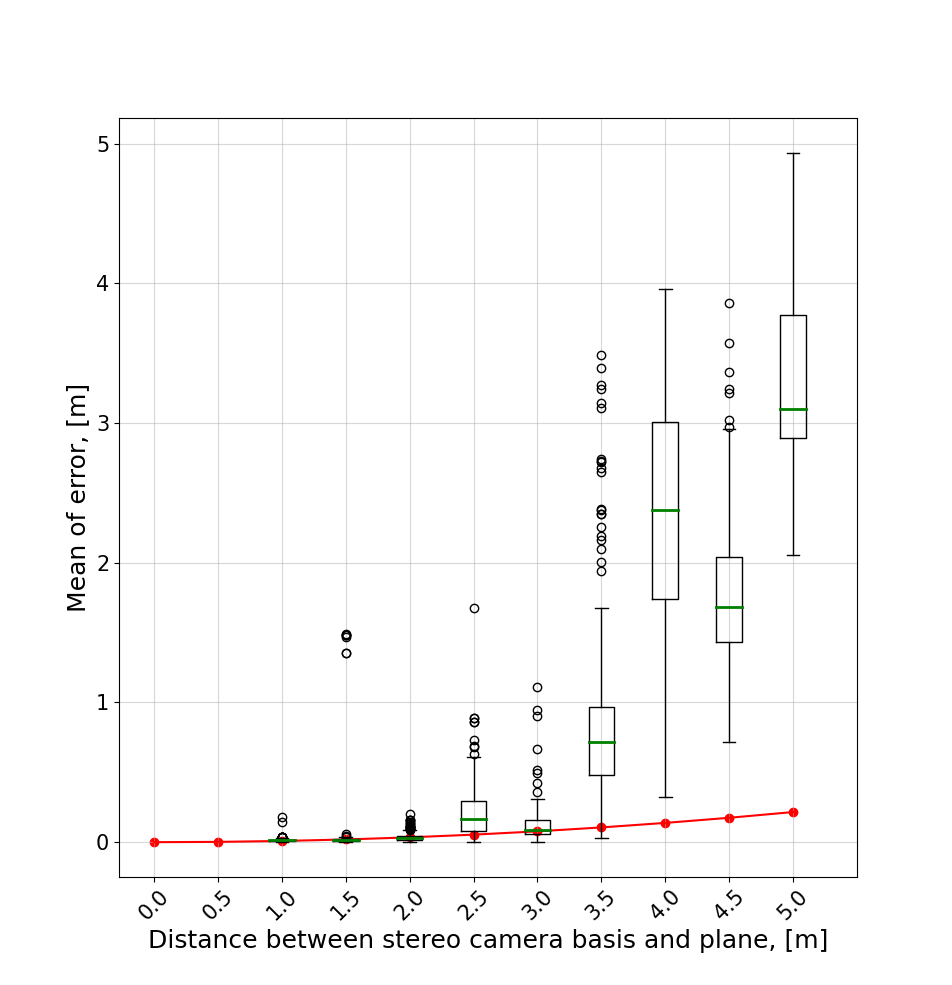
\includegraphics[width=\textwidth]{graphics/experiment_1_general.png}
    \caption[The first experiment results.]{The first experiment results. The red line represents the theoretical error for the given setup. 
        Green lines represents the median for each $n$ measurements at a distance $d$. 
        A box marks an interval from the first quartile to the third quartile.
        The whiskers go from each quartile of the measured values to the lower and upper fences.
        Black points represents outliers.
    }
    \label{fig:exp_1_chart_dists}
  \end{subfigure}
  \hfill
  \begin{subfigure}[ht]{0.49\textwidth}
    \centering
    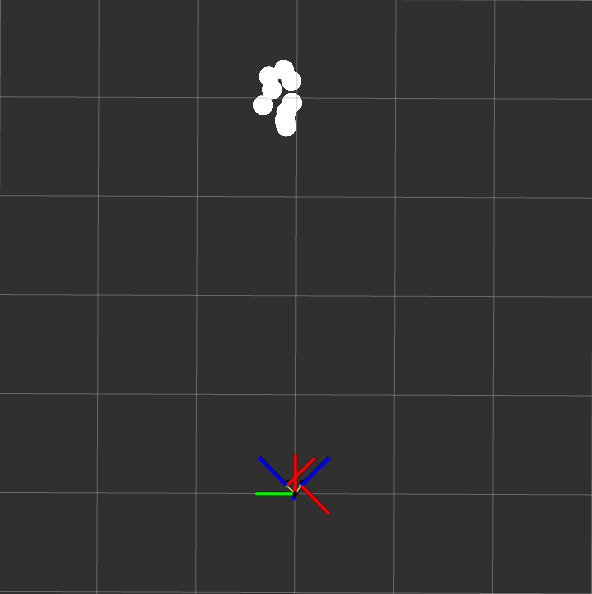
\includegraphics[width=\textwidth]{graphics/experiment_1_4m.png}
    \caption[Top view of the experiment.]{Top view of the experiment. 
    The grid's cell size is $1$m$\times$$1$m.
    The colored axes represent the stereo pair's coordinate system.
    Red color stands for $X$ axis, green for $Y$ and blue for $Z$.
    The point cloud (white dots) represents the 3D points reconstructed from feature points seen by both cameras.}
    \label{fig:exp_1_topview}
  \end{subfigure}
  \caption{Results from the first experiment: distance to the estimated plane.}
  \label{fig:exp_1_exp}
\end{figure}

\begin{figure}[ht]
    \centering
    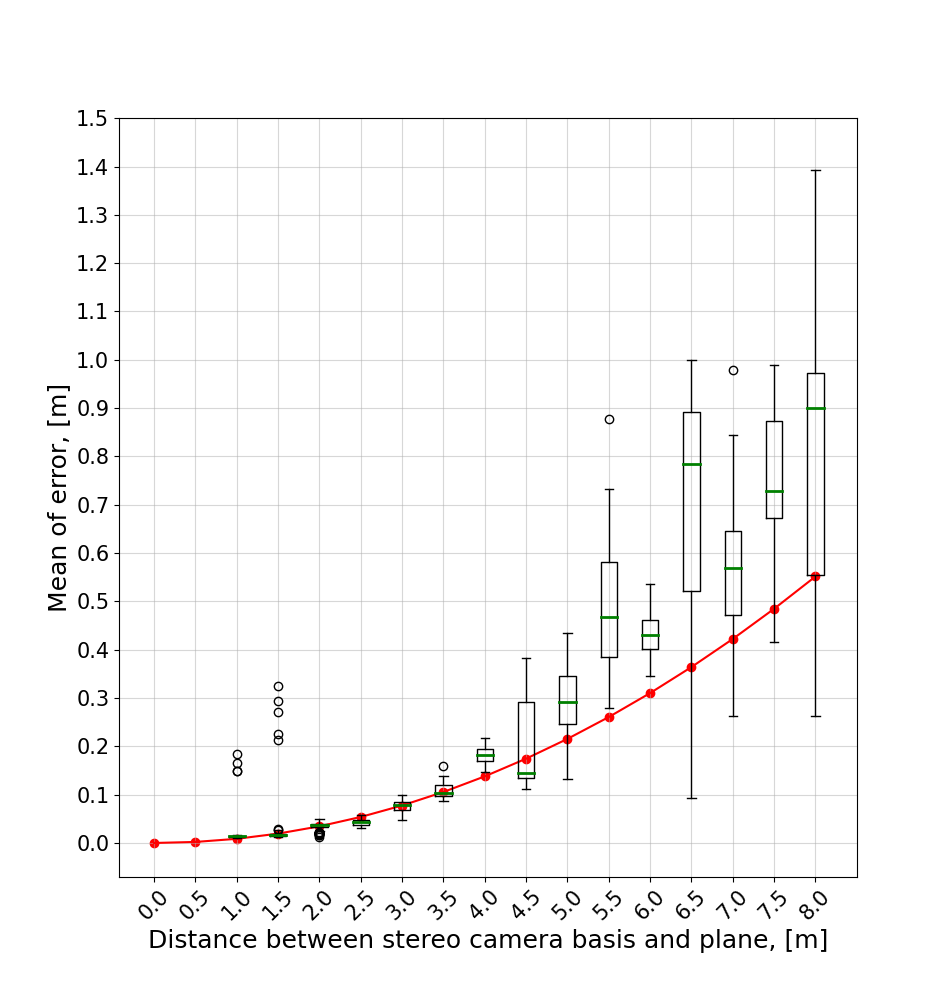
\includegraphics[width=\textwidth]{graphics/experiment_2_general.png}
    \caption[Results from the second experiment.]{Results from the second experiment.
    The Red line represents the theoretical error for the given setup.
        Green lines represents the median for each $n$ measurements at a distance $d$. 
        A box marks an interval from the first quartile to the third quartile.
        The whiskers go from each quartile of the measured values to the lower and upper fences.
        Black points represents outliers.
    }
    \label{fig:exp_2_general}
\end{figure}

The reprojection error is not a good metric to evaluate the triangulation performance because with increasing distance of objects in the environment, the corresponding feature points are closer together in the image (see \autoref{fig:exp_1_disparity}), and the reprojection error decreases (see \autoref{fig:exp_1_repro}).
To measure the quality of distance estimation, a different approach was chosen.
A pattern with multiple features was attached to a white wall in a corridor within a featureless environment.
The camera prototype on a tripod was placed at different distances from the wall and was set up so that its $Y-Z$ plane was parallel to the wall as in \autoref{fig:exp_process}.
Based on this, we assume that the ground-truth position of all observed 3D points lies on a plane whose orientation and distance from the coordinate frame's origin are known.
Then, several measurements were made, and the obtained data were collected and saved to post-process it separately, analyse and obtain plots.

Let us define the wall plane as $\Omega$, the distance from the origin of the stereo pair's common frame to the wall as $d$, an estimated plane as $\Omega'$ and an estimated distance to the plane as $d'$.
The main goal of the experiments was to measure the precision of triangulation and compare it with the theoretical error, introduced in \cite{cv_theoretical_error} as a function of the distance based on the geometrical and optical parameters of the setup.
The theoretical error is defined as
\begin{equation}
    e_Z = \frac{Z^2 \delta}{bf},
\end{equation}
where $Z$ is the real distance, $\delta$ is the matching error in pixels, $f$ is the focal length and $b = \lVert \vec{b} \rVert$ (see \autoref{fig:sch_stereo}).
To compute the theoretical error for the current prototype, the following values was used: $\delta=1$px, $f=38$mm and $b=14.5$mm.

\subsection{Distance to an estimated plane}
\label{sec:exp1}
To find the distance $d'$, $\Omega'$ should be estimated using the triangulated feature points.
In this experiment, for each set of 3D points corresponding to a specific distance $d$, $\Omega'$ is estimated using RANSAC to filter outliers (an implementation from PCL was used).
The error is defined as
\begin{equation}
    e = \frac{1}{k}\sum_{j=0}^{k}{|d - d'_j|},
\end{equation}
where $d'_j$ is the estimated distance to $\Omega'$ for each measurement and $k$ is the number of measurements.

In this experiment, the absolute error $e$ was measured for each distance $d$ from $1$m to $5$m with a step of $0.5$m.
The result of this experiment is shown in \autoref{fig:exp_1_chart_dists}.
According to the figure, the distance deviates significantly after $3$m, and the error grows much faster than the theoretical caused by the camera's limited resolution.
In \autoref{fig:exp_1_topview} a top view of the experiment is shown for $d=4$m.
It can be seen that the plane can not be estimated correctly at this distance using RANSAC anymore because of too large error in distance estimation for each triangulated point.

\subsection{Distance to a predefined plane}
\label{sec:exp2}
With increasing the distance $d$, feature points become less distinguishable due to the limited resolution of the camera.
The estimated plane $\Omega'$ is inaccurate from a certain distance because of high noise in the $X$ direction of the points and low spread of the points in the $Y-Z$ direction (see \autoref{fig:exp_1_topview}), but still, the points are close to the actual plane $\Omega$.
That is why the second experiment was constructed.

The experiment was done using the same setup as described in \autoref{sec:eval_setup}. 
The difference is that $\Omega'$ is not estimated using the least squares RANSAC method to fit the plane to the points, but as the plane parallel to $\Omega$ on a distance $e'_i$, that is defined as
\begin{equation}    
    e' = \frac{1}{k} \sum_{j=0}^{k}{|p'_j|},
\end{equation}
where $k$ is the number of measurements and $|p'_j|$ is the absolute distance from point $\vec{p}'_j$ to $\Omega$.

% In \autoref{fig:exp_2_general} the red line represents the theoretical error for the proposed setup.

The ground-truth distance $d$ for the current experiment was from $1$m to $8$m as the maximum distance at which key points can be detected (empirically found) with a $0.5$m step.
The result of the second experiment is shown in \autoref{fig:exp_2_general}, where the measured error corresponds to the theoretical error up to $d=4$ meters with a small deviation. 
After $4$m, the difference between the theoretical and measured error grows larger with a larger variance.
One possible cause of this difference is that there is an error in camera calibration and fixed focal length, so detected patterns on longer distances are blurred and less accurate. 

\section{Rate testing}
To ensure that the obstacle detection is practical for real-world deployment, not only triangulation quality is important, but also the rate at which the MAV can receive the data from the obstacle avoidance module and the delay of the data.
The data rate, maximal and minimal delays averaged over $5\,$min are shown in \autoref{tab:eval_freq}.
\begin{table}[ht]
    \begin{center}
      \begin{tabular}{ll}
      \hline
        Parameter & Value \\
        Minimal delay &  0.042\,s \\
        Maximal delay &  0.196\,s \\
        Average rate & 10.607\,Hz \\ 
      \end{tabular}
    \end{center}
    \caption{Measured data delay and rate of the proposed system.}
    \label{tab:eval_freq}
\end{table}
 
\section{Experiments summary}
The quality of the distance estimation to obstacles was demonstrated in the two experiments.
The first experiment, described in \autoref{sec:exp1}, shows that the precision of the proposed method is relatively high for distances up to $3\,$m, and the second experiment, described in \autoref{sec:exp2} provided further insight into the statistics of the error over longer distances. 
The estimated distance error on $3$m is less than $3\%$.
The maximum distance at which 3D points could be reliably estimated is $8$m with an error of up to $1$m.
On longer distances, feature points can not be reliably detected anymore.
The proposed solution works with an average frequency of $10$Hz.
